\chapter{Analisis}
\label{chap:analisis}

Pada bab ini dijelaskan mengenai ....

\section{Analisis Perangkat Lunak Serupa}
\label{sec:mpYangSudahAda}

Pada tahun 2008, Pisceldo dkk pernah membuat sebuah artikel yang berjudul "A Two-Level Morphological Analyser for the Indonesian Language"\cite{manurung:08:indonesian}. Artikel ini berisi tentang usaha pembuatan perangkat lunak \textit{morphological analyser} untuk bahasa Indonesia melalui pendekatan \textit{two-level}. Perangkat lunak ini dapat memproses kata yang merupakan hasil afiksasi dan reduplikasi. 

Proses morphological analysis mengambil informasi berupa kategori gramatikal dari sebuah kata berdasarkan aturan morfologi yang ada. Pada penelitian ini dipakai \textit{two-level morphology approach}, prosesnya dipecah menjadi menentukan aturan morfotaktik dan morfofonemik. Aturan ini dimodelkan ke dalam network \textit{finite-state transducers} dan diimplementasikan dengan \textbf{xfst} dan \textbf{lexc}. Sistem yang dihasilkan dari penelitian ini bisa menangani reduplikasi, proses morfologi yang tidak memerlukan penggabungan kata (non-concatenative).

\subsection{Desain}
\label{sec:desainMPYangSudahAda}

Desain perangkat lunak dibagi dalam dua komponen:
	\begin{itemize}
		\item Morfotaktik: menentukan kelas morfem mana yang bisa mengikuti kelas morfem lain dalam sebuah kata
		\item Morfofonemik: memodelkan perubahan fonologi yang terjadi pada proses pembentukan kata
	\end{itemize}

Adapun desain leksikon yang digunakan terdiri dari 4 kelas yaitu verbs, nouns, adjectives, dan 'etc' (pronouns, adverbs, numbers, dan particles)

Desain tag yang digunakan:
	\begin{itemize}
		\item Normal tags: $+VERB, +NOUN, +ADJ, +BAREVERB, +BARENOUN, +BAREADJ, \\+BAREETC, +AV, +PASS, +UV,$ dan $+REDUP$
		\item Special tags: $+CAUS\_KAN, +APPL\_KAN, +CAUS\_I, +APPL\_I, +ACTOR, \\+INSTRUMENT$
	\end{itemize}
	
Detailnya adalah sebagai berikut:
	\begin{itemize}
		\item Tag seperti $+VERB, +NOUN$, dan $+ADJ$ menandai kata yang sudah melalui proses morfologi
		\item Tag seperti $+BAREVERB, +BARENOUN, +BAREADJ,$ dan $+BAREETC$ menandai kata dasar
		\item Tag seperti $+AV, +PASS,$ dan $+UV$ menandai kategori gramatikal, $+AV$ untuk active voice, $+PASS$ untuk passive voice, dan $+UV$ untuk undergoer voice
		\item Tag $+REDUP$ untuk menandai reduplikasi
		\item Tag $+CAUS\_KAN, +APPL\_KAN, +CAUS\_I$, dan $+APPL\_I$ menandai kata tersebut merupakan causative atau applicative dengan melihat akhirannya
		\item Tag $+ACTOR$ dan $+INSTRUMENT$ menandai kata tersebut membawa makna actor atau instrument
	\end{itemize}
	
Aturan morfotaktik untuk bahasa Indonesia ada 13 aturan, 10 aturan untuk pembubuhan afiks (meN-, peN-, di-, per-, ber-, ter-, ke-, -an, -kan, dan -i), dan 3 aturan untuk reduplikasi (utuh, sebagian, berimbuhan).

Contoh aturan morfotaktik pembubuhan afiks:
	\begin{itemize}
		\item membersihkan (meN+bersih+kan). Kata bersih adalah adjective, setelah digabung dengan meN-kan hasilnya adalah verb.
		\item pembelajaran (peN+ber+ajar+an). Kata ajar adalah verb, setelah digabung dengan peN-ber-an, hasilnya adalah noun.
		\item keberhasilan (ke+ber+hasil+an). Kata hasil adalah noun, setelah digabung dengan ke-ber-an, hasilnya tetap noun.
		\item terangi (terang+i). Kata terang adalah adjective, setelah digabung dengan -i, hasilnya adalah verb.
	\end{itemize}

Contoh aturan morfotaktik reduplikasi:
	\begin{itemize}
\item buku-buku. Kata buku-buku, adalah noun, dihasilkan dari kata buku, yang juga adalah sebuah noun.
\item kekayaan-kekayaan (reduplikasi dari ke+kaya+an). Kata kaya adalah adjective. Setelah mengalami proses morfologi, hasilnya adalah noun.
\item berlari-lari (ber+lari-lari). Kata lari adalah verb. Setelah mengalami proses morfologi, hasilnya adalah juga verb.
\item tanam-menanam (tanam-meN+tanam). Kata tanam adalah verb. Setelah mengalami proses morfologi, hasilnya adalah juga verb.
	\end{itemize}

Selama tahap penerapan aturan morfotaktik, ada beberapa langkah yang harus dilakukan, yaitu penambahan prefiks dan preprefiks, penambahan stems dan part-of-speech, penambahan sufiks, dan proses akhir berupa penambahan tags.

Aturan morfofonemik untuk bahasa Indonesia dibagi dalam dua kelompok, ada 4 aturan untuk memodelkan perubahan pada kata dasar dan ada 7 aturan untuk memodelkan perubahan pada afiks.

Aturan pada perubahan kata dasar:
	\begin{itemize}
		\item Mengganti /k/ menjadi /ng/ jika mendapat awalan meN- atau peN-.
Contoh: meN+kantuk menjadi mengantuk.
		\item Mengganti /s/ menjadi /ny/ jika mendapat awalan meN- atau peN-.
Contoh: peN+sebaran menjadi penyebaran.
		\item Mengganti /p/ menjadi /m/ jika mendapat awalan meN- atau peN-.
Contoh: peN+pakai menjadi pemakai.
		\item Mengganti /t/ menjadi /n/ jika mendapat awalan meN- atau peN-.
Contoh: meN+tertawakan menjadi menertawakan.
	\end{itemize}

Aturan pada perubahan afiks:
	\begin{itemize}
		\item Penghapusan /N/ jika awalan meN- diikuti /l/, /m/, /n/, /r/, /y/, /w/, /t/, /s/, /p/, /k/ atau jika awalan peN diikuti /l/, /m/, /n/, /r/, /d/, /w/, /t/, /s/, /p/, /k/. 
Contoh: meN+lukis menjadi melukis.
		\item Penghapusan /r/ jika awalan ber-, ter-, atau per- diikuti oleh /r/ atau kata yang suku pertamanya berakhir dengan /er/. 
Contoh: ber+runding menjadi berunding.
		\item Penggantian /N/ dengan /n/ jika meN- diikuti oleh /d/, /c/, /j/, /sy/ atau jika peN- diikuti /d/, /c/, /j/. 
Contoh: peN+jual menjadi penjual.
		\item Penggantian /N/ dengan /m/ jika meN- atau peN- diikuti oleh /b/, /f/. 
Contoh: peN+buru menjadi pemburu.
		\item Penggantian /N/ dengan /nge/ jika meN- diikuti oleh kata dengan satu suku. 
Contoh: meN+rem menjadi mengerem.
		\item Penggantian /N/ dengan /l/ jika peN- diikuti dengan kata ajar. 
Contoh: peN+ajar menjadi pelajar.
		\item Penggantian /r/ dengan /l/ jika ber- diikuti dengan kata ajar. 
Contoh: ber+ajar menjadi belajar.
	\end{itemize}

Desain dari aturan morfofonemik untuk reduplikasi secara umum sama dengan afiksasi karena proses morfofonemik pada reduplikasi terjadi saat proses afiksasi dilakukan.

Pada kasus di mana perubahan terjadi pada afiks dan kata dasar sekaligus, perlu ada beberapa penyesuaian aturan untuk digunakan pada bentuk reduplikasi. Contoh pada aturan morfofonemik penggantian /k/ menjadi /ng/ dan penghapusan /N/ yang bekerja bersamaan, awalnya adalah penghapusan /k/ dan penggantian /N/ dengan /ng/. Namun, pendekatan ini tidak bekerja jika melibatkan reduplikasi. Kata mengotak-ngotakkan tidak akan dianalisis dengan tepat jika morphological analyser menggunakan aturan penghapusan /k/ dan penggantian /N/ dengan /ng/. Kata mengotak-ngotakkan dihasilkan dari kata dasar kotak yang dimodifikasi dengan reduplikasi berafiks meN-kan. Jika penghapusan /k/ dan penggantian /N/ dengan /ng/ digunakan, hasil dari proses tersebut adalah kata mengotak-otakkan yang mana tidak valid. Ini adalah alasan dalam reduplikasi aturannya diubah menjadi penggantian /k/ menjadi /ng/ dan penghapusan /N/ sehingga dihasilkan kata mengotak-ngotakkan.

\subsection{Implementasi}
\label{sec:implementasiMPYangSudahAda}

Morphological analyser bahasa Indonesia ini diimplementasikan menggunakan \textbf{xfst} and \textbf{lexc}. Aturan morfotaktik diimplementasikan dengan \textbf{xfst} sementara aturan morfofonemik diimplementasikan dengan \textbf{lexc}.

Implementasi aturan morfotaktik dapat diilustrasikan dengan \textit{finite-state automata} yang ditunjukkan pada gambar \ref{gambar-fsa-morfotaktik}. Kata bahasa Indonesia yang valid, yaitu yang dihasilkan melalui proses morfologi yang benar, dapat diterima oleh automata, sementara yang tidak valid ditolak.

Berawal dari root, setiap state menentukan kemungkinan lanjutan state selagi mengambil simbol tertentu. Dalam \textbf{lexc}, state ini disebut \textit{continuation classes}. Semua continuation classes yang bisa dicapai dari root menampilkan prefiks dan preprefiks. Perbedaan di antara keduanya diperlukan untuk mengenali variasi morfologi berupa adanya 2 prefiks, seperti prefiks memper-, diper-. Dari sana, continuation class selanjutnya adalah stem, di mana kata dasar diambil. Ini diteruskan dengan beberapa classes yang menampilkan kemungkinan sufiks, namun ada juga class Redup1 dan Redup2 yang muncul sebelum dan setelah sufiks. Fungsinya adalah untuk menangani reduplikasi. Terakhir, tagEmit class memproses semua tags yang belum ditangani oleh class sebelumnya.

\begin{figure}[H]
\centering
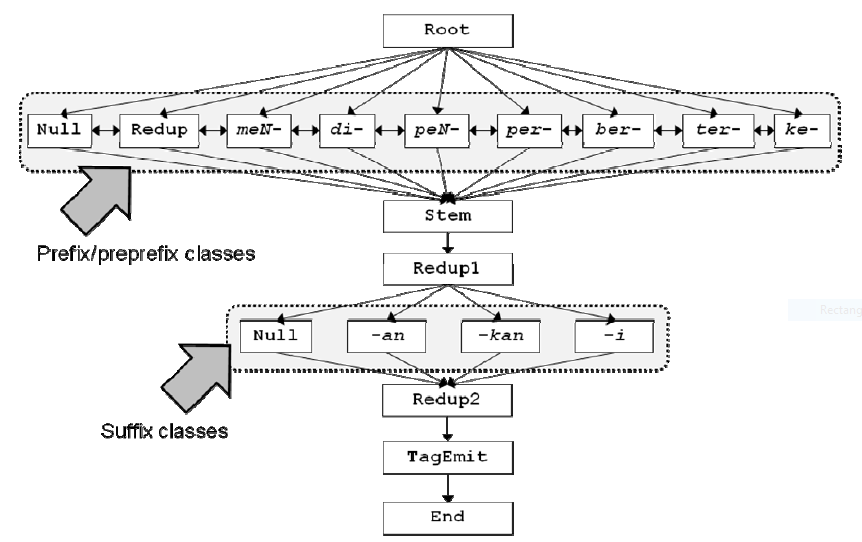
\includegraphics[scale=0.5]{Gambar/gambar-fsa-morfotaktik}
\caption[Ilustrasi proses morfotaktik]{Ilustrasi proses morfotaktik\cite{manurung:08:indonesian}} 
\label{gambar-fsa-morfotaktik}
\end{figure}

%Selama proses morfotaktik ini, kita menggunakan flag diacritics, fitur penting dari \textbf{lexc} yang memperkirakan kemampuan dari struktur fitur, di antaranya mampu menentukan hambatan tertentu untuk memastikan hanya jalur yang valid dari network yang dilewati. Satu keuntungan dari pendekatan ini adalah perbaikan dari representasi network yang ringkas. Ada 3 flag diacritics yang digunakan dalam model kita: positive setting (@P.feat.val@), required test (@R.feat.val@), dan disallow test (@D.feat.val@). Dengan menggunakan diacritics ini, kita dapat menetapkan nilai dan hambatan dari aspek tertentu, yang harus konsisten sepanjang jalur.

%Sebagai contoh, prefiks meN- bisa dikombinasikan dengan sufiks -kan dan -i, tapi tidak -an. Kita dapat menampilkan ini dengan fitur, misal PREF, yang dipasangkan pada meN pada (pre)prefix state (@P.PREF.meN@). Tes yang cocok selanjutnya ditambahkan pada suffix states, misal jalur saat ini melewati prefix state meN-, @R.PREF.meN@ menetapkan ada sufiks yang harus dipasangkan, sementara @D.PREF.meN@ mencegah sufiks diterapkan.

Sudah dibahas di atas bahwa morfologi bahasa Indonesia mengandung proses reduplikasi. Sangat sulit menangani ini dengan regular grammar yang diimplementasikan dengan finite-state automata. Oleh karena itu, digunakan fitur compile-replace dalam \textbf{xfst}. Fitur ini memperbolehkan pengulangan bahasa yang kompleks dengan menggunakan tanda $"^{\wedge}["$ dan $"^{\wedge}]"$ untuk menandai bagian reduplikasi. Tanda kurung siku kanan juga ditambah dengan $^{\wedge}2$ untuk menandakan duplikasi; sehingga lengkapnya adalah $"^{\wedge}["$ dan $"^{\wedge}2^{\wedge}]"$. Dengan definisi network ini, \textbf{xfst} melakukan compiles dan post-processes dari keterangan ini untuk menghasilkan network baru yang bisa mengenali reduplikasi. Contoh, $"^{\wedge}[buku^{\wedge}2^{\wedge}]"$ akan dicompile menjadi bukubuku.

Idenya adalah untuk memasukkan $"^{\wedge}["$ dan $"^{\wedge}2^{\wedge}]"$ pada posisi yang tepat. Karena banyaknya tipe reduplikasi dalam bahasa Indonesia, aturan reduplikasi dapat ditemukan pada state Redup (pre)prefix dan state Redup1 dan Redup2. State prefix Redup mengambil tanda kurung siku $"^{\wedge}["$ dan mengeset flag yang tepat sebagai pengingat bahwa tanda kurung siku kanan dibutuhkan. State Redup1 bertanggung jawab untuk menutup reduplikasi sebagian dan reduplikasi berafiks, contoh di mana sufiks tidak diikutkan dalam reduplikasi, sementara state Redup2 bertanggung jawab untuk menutup reduplikasi utuh, contoh di mana sufiks menjadi bagian dari proses reduplikasi. Baik state Redup1 dan Redup2 mengecek nilai dari flag REDUP yang diset pada prefix state Redup.

Transducer yang utuh terdiri dari aturan morfotaktik dan morfofonemik sehingga keluaran dari implementasi aturan morfotaktik menjadi masukan bagi implementasi aturan morfofonemik. Dari contoh sebelumnya, keluaran dari implementasi aturan morfotaktik adalah me$^{\wedge}$Npukuli dan menjadi masukan bagi implementasi aturan morfofonemik.

Berbeda dengan implementasi aturan morfotaktik yang bisa direpresentasikan dengan diagram alur proses, implementasi dari aturan morfofonemik berisi aturan-aturan perubahan dan penggantian fonem seperti yang sudah dipaparkan sebelumnya. Pada gambar \ref{gambar-implementasi-aturan-morfofonemik} berikut adalah contoh implementasi dari aturan 'RG4' yang mengkodekan penghapusan /N/ dan penggantian 4 jenis fonem pada kata dasar:

\begin{figure}[H]
\centering
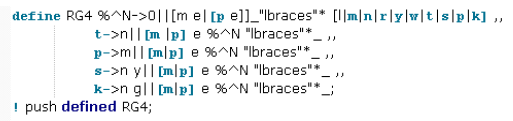
\includegraphics[scale=0.6]{Gambar/gambar-implementasi-aturan-morfofonemik}
\caption[Implementasi aturan morfofonemik]{Implementasi aturan morfofonemik\cite{manurung:08:indonesian}} 
\label{gambar-implementasi-aturan-morfofonemik}
\end{figure}

Aturan ini terdiri dari 5 aturan yang bekerja secara paralel. Aturan pertama adalah penghapusan /N/ pada prefiks jika /me/ atau /pe/ diikuti oleh kata dasar dengan fonem awal /l/, /m/, /n/, /r/, /y/, /w/, /t/, /s/, /p/, atau /k/.

Aturan selanjutnya terdiri dari 4 aturan perubahan fonem awal pada kata dasar yang diberikan prefiks /me$^{\wedge}$N/ atau /pe$^{\wedge}$N/, dan fonem awal pada kata dasarnya adalah /t/, /p/, /s/, atau /k/. Lebih detail, fonem /t/ akan diganti dengan /n/, fonem /p/ diganti dengan /m/, fonem /s/ diganti dengan /ny/, dan fonem /k/ diganti dengan /ng/.

Contoh masukan me$^{\wedge}$Npukuli pada proses sebelumnya memenuhi aturan penghapusan /N/ dan penggantian fonem awal /p/ dari kata dasar dengan fonem /m/. Kata me$^{\wedge}$Npukuli akan diproses menjadi kata memukuli. Kata tersebut merupakan kata yang valid dalam bahasa Indonesia dan proses berakhir di sini.

Pengujian dilakukan dengan menjalankan tes kasus dengan kata yang diambil dari Kamus Besar Bahasa Indonesia versi elektronik. Pengujian dilakukan pada implementasi dari aturan morfotaktik dan morfofonemik secara terpisah. Untuk menguji kemampuan dari analyser untuk menerima masukan yang valid dan tidak valid, tes kasus yang digunakan mengandung penulisan kombinasi morfem yang valid dan tidak valid. Hasil dari pengujian ditampilkan pada tabel \ref{tabel-hasil-pengujian-morfotaktik}, yang menunjukkan hasil pengujian morfotaktik, dan tabel \ref{tabel-hasil-pengujian-morfofonemik}, yang menunjukkan hasil pengujian morfofonemik. Kolom Analisis menampilkan hasil dari sistem yang memproses penguraian struktur morfologi dari kata dalam bahasa Indonesia. Contoh, diberikan masukan kata memukul, sistem diharapkan menghasilkan keluaran pukul+Verb+AV. Sementara, kolom Sintesis menangani situasi yang sebaliknya, di mana masukannya adalah tag morfologi dan sistem diharapkan menghasilkan keluaran berupa kata yang valid dalam bahasa Indonesia.

\begin{table}[H]
\centering
\begin{tabular}{|c|c|c|c|}
\hline
\textbf{Hasil} & \textbf{Analisis} & \textbf{Sintesis} & \textbf{Jumlah} \\
\hline
1. Hasil benar & 103 & 43 & 146 \\
\hline
2. Beberapa hasil, ada yang benar & 46 & 106 & 152 \\
\hline
3. Hasil salah & 3 & 3 & 6 \\
\hline
\textbf{Jumlah} & 152 & 152 & 308 \\
\hline
\end{tabular}
\caption{Hasil pengujian morfotaktik\cite{manurung:08:indonesian}}
\label{tabel-hasil-pengujian-morfotaktik}
\end{table}

\begin{table}[H]
\centering
\begin{tabular}{|c|c|c|c|}
\hline
\textbf{Hasil} & \textbf{Analisis} & \textbf{Sintesis} & \textbf{Jumlah} \\
\hline
1. Hasil benar & 51 & 21 & 72 \\
\hline
2. Beberapa hasil, ada yang benar & 6 & 36 & 42 \\
\hline
3. Hasil salah & 1 & 1 & 2 \\
\hline
\textbf{Jumlah} & 58 & 58 & 116 \\
\hline
\end{tabular}
\caption{Hasil pengujian morfofonemik\cite{manurung:08:indonesian}}
\label{tabel-hasil-pengujian-morfofonemik}
\end{table}

Ada tiga kategori hasil pengujian, kategori pertama adalah ketika sistem menghasilkan sebuah hasil analisis atau sintesis yang benar atau tidak menghasilkan apapun untuk tes kasus yang tidak valid. Kategori kedua adalah ketika sistem diberikan masukan valid dan menghasilkan beberapa jawaban, yang salah satunya adalah jawaban yang diharapkan. Terakhir, kategori ketiga adalah ketika sistem gagal menganalisis atau menyintesis tes kasus yang valid atau tidak memproduksi jawaban yang tepat ketika diberikan tes kasus yang tidak valid.

Dari tabel, dapat dilihat bahwa hasil untuk proses analisis lebih baik dari proses sintesis, di mana sistem cenderung memproduksi lebih dari satu kemungkinan jawaban. Contoh, sistem ini mampu menghasilkan kata memukul pada proses analisis, namun ketika proses sintesis untuk pukul+Verb+AV, sistem menghasilkan beberapa kemungkinan jawaban yaitu memukulkan, memperpukuli, mengepukulkan, dll. Ini menandakan diperlukan tag yang lebih baik untuk fitur morfologi.

\section{Leksikon}
\label{sec:leksikon}
Leksikon, seperti dijelaskan pada subbab \ref{sec:morfemDasarDLL}, dapat dipadankan dengan istilah \textit{kosakata} atau \textit{perbendaharaan kata}. Leksikon dibutuhkan pada proses \textit{morphological parsing} untuk mengetahui apakah sebuah kata yang sedang diproses adalah sebuah bentuk dasar yang valid atau tidak dalam bahasa Indonesia. Leksikon menyimpan kumpulan bentuk dasar dan turunannya untuk nantinya diakses ketika proses \textit{morphological parsing} dilakukan.

Leksikon dalam proses \textit{morphological parsing} harus bisa diakses dengan cepat dan efektif. Hal ini dikarenakan leksikon akan diakses sangat sering dalam proses ini. Leksikon akan diakses sekitar 3-5 kali untuk setiap kata yang sedang diproses. Oleh karena itu, leksikon perlu disimpan pada struktur data yang memungkinkan waktu akses yang cepat supaya keseluruhan proses dapat dijalankan dalam waktu yang masuk akal. 

Struktur data yang saat ini terkenal paling cepat untuk diakses adalah struktur data \textit{trie}. Trie adalah struktur data berbentuk pohon yang menyimpan himpunan string yang jika ditelusuri setiap node mulai dari akar hingga daun akan membentuk suatu string yang merupakan kunci yang kita cari. Setiap string yang dihasilkan dari node awal yang sama akan mempunyai awalan (prefiks) yang sama, karena itulah trie disebut juga pohon prefiks.

\begin{figure}[H]
\centering
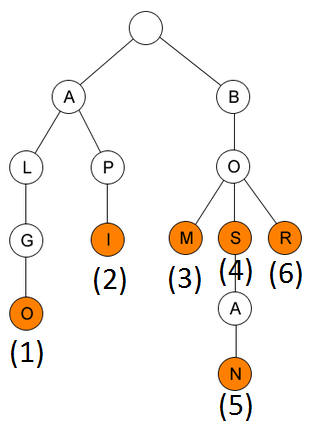
\includegraphics[scale=0.75]{Gambar/gambar-trie}
\caption[Struktur data trie]{Struktur data trie} 
\label{bagan-trie}
\end{figure}

Struktur data trie yang digambarkan pada bagan \ref{bagan-trie} menyimpan enam string kunci dari dua buah awalan, yaitu string "A" dan "B". Jika kita telusuri dari node akar "A" sampai node daun "O", kita akan mendapat string "ALGO" yang ditandai dengan nomor (1). String lain yang disimpan pada contoh tersebut adalah string "API" pada nomor (2), string "BOM" pada nomor (3), string "BOS" pada nomor (4), string "BOSAN" pada nomor (5), dan string "BOR" pada nomor (6).

Perlu diperhatikan bahwa sebuah string kunci tidak harus disimpan dengan node terakhir ada pada posisi daun, seperti pada string "BOS" pada nomor 4. Node terakhir pada string tersebut merupakan node internal. Penyimpanan seperti ini bisa dilakukan dengan menandai setiap node yang merupakan akhir dari sebuah string yang membentuk kata.

Kata yang disimpan dalam leksikon terdiri dari dua jenis kata, yaitu kata dasar dan kata turunan. Contoh kata dasar adalah kata 'makan', 'sapu', dan 'kerja' sementara contoh kata turunan adalah kata 'makan-makan', 'menyapu', dan 'kerja bakti'. Kata-kata turunan disimpan sebagai bagian dari kata dasar dan dapat diakses ketika dibutuhkan. Dalam Kamus Besar Bahasa Indonesia Dalam Jaringan (KBBI daring)\footnote{https://kbbi.kemdikbud.go.id/}, kata dasar dan kata turunan disimpan secara terpisah namun keduanya dapat diakses melalui cara yang sama, yaitu dengan menuliskannya pada kolom pencarian. Sementara pada Kamus Besar Bahasa Indonesia Luar Jaringan (KBBI luring)\footnote{http://ebsoft.web.id/kbbi-kamus-besar-bahasa-indonesia-offline-gratis/}, hanya kata dasar saja yang bisa diakses dengan menuliskannya pada kolom pencarian. Pada penelitian kali ini akan digunakan struktur penyimpanan seperti pada KBBI luring.

Struktur penyimpanan seperti pada KBBI luring memungkinkan untuk mengenali perbedaan antara kata dasar dan kata yang telah melalui proses morfologi seperti afiksasi, reduplikasi, dan komposisi. Perangkat lunak yang dirancang pada penelitian ini harus dapat menentukan apakah sebuah kata merupakan kata dasar yang valid dalam bahasa Indonesia.


\section{Proses \textit{Morphological Parsing}}
\label{sec:morphologicalParsing}

Pada subbab \ref{sec:prosesMorfologi} telah dibahas mengenai proses morfologi, yang pada dasarnya adalah proses pembentukan kata melalui beberapa proses, yaitu pembubuhan afiks (afiksasi), pengulangan (reduplikasi), penggabungan (komposisi), pemendekan (akronimisasi), dan pengubahan status (konversi). Proses \textit{morphological parsing} merupakan kebalikan dari proses morfologi. Masukan bagi proses \textit{morphological parsing} adalah kata atau kalimat yang telah melalui proses morfologi dan keluarannya adalah komponen-komponen penyusunnya.

Proses \textit{morphological parsing} untuk setiap kata dalam masukan dapat dituliskan sebagai berikut:
\begin{enumerate}
	\item Periksa leksikon, jika kata tersebut ada dalam leksikon, masukkan sebagai salah satu kemungkinan keluaran
	\item Periksa adanya simbol penghubung (-), yang menandakan hasil proses reduplikasi, lalu lakukan pemisahan kata dan lakukan proses parsing pada kedua kata tersebut
	\item Jika ada kata yang mengikuti, periksa kemungkinan kata yang sedang diproses dan kata yang mengikuti adalah dua kata hasil komposisi, lalu lakukan proses parsing pada kedua kata tersebut
	\item Periksa adanya kemungkinan afiks, baik itu prefiks, sufiks, infiks, maupun konfiks. Pisahkan afiks yang ditemukan dengan komponen kata yang lain dan lakukan pengecekan leksikon pada komponen kata tersebut
	\item Jika sudah dilakukan pemisahan terhadap kemungkinan afiks namun kata yang sedang diproses tidak ditemukan dalam leksikon, kemungkinan kata tersebut bukan kata dalam bahasa Indonesia
\end{enumerate}

Sebagai contoh, jika dilakukan proses \textit{morphological parsing} pada kata 'kemerah-merahan', maka prosesnya adalah sebagai berikut:
\begin{itemize}
	\item Periksa leksikon, kata tersebut tidak ditemukan dalam leksikon
	\item Ditemukan simbol penghubung (-) sehingga diketahui kata tersebut adalah hasil proses reduplikasi. Pisahkan kata sehingga didapat kata 'kemerah' dan 'merahan'
	\item Periksa leksikon kembali untuk kedua kata tersebut, kedua kata tersebut tidak ditemukan dalam leksikon
	\item Periksa kemungkinan afiks pada kata 'kemerah' dan 'merahan'
	\item Didapatkan prefiks $\lbrace$ke-$\rbrace$ + bentuk dasar $\lbrace$merah$\rbrace$ dan bentuk dasar $\lbrace$merah$\rbrace$ + sufiks $\lbrace$-an$\rbrace$, yang setelah ditinjau lebih lanjut didapatkan konfiks $\lbrace$ke-an$\rbrace$ + bentuk dasar $\lbrace$merah$\rbrace$
	\item Hasil akhir proses parsing adalah konfiks $\lbrace$ke-an$\rbrace$ + bentuk dasar $\lbrace$merah$\rbrace$ + reduplikasi
\end{itemize}

Walaupun berbentuk mirip dengan kata 'kemerah-merahan', proses parsing pada kata 'berlari-larian' sedikit berbeda. Prosesnya adalah sebagai berikut:
\begin{itemize}
	\item Periksa leksikon, kata tersebut tidak ditemukan dalam leksikon
	\item Ditemukan simbol penghubung (-) sehingga diketahui kata tersebut adalah hasil proses reduplikasi. Pisahkan kata sehingga didapat kata 'berlari' dan 'larian'
	\item Periksa leksikon kembali untuk kedua kata tersebut, kata 'berlari' ditemukan sebagai turunan dari kata dasar $\lbrace$lari$\rbrace$ yang ditambahkan prefiks $\lbrace$ber-$\rbrace$
	\item Periksa kemungkinan afiks pada kata 'larian'
	\item Didapatkan bentuk dasar $\lbrace$lari$\rbrace$ + sufiks $\lbrace$-an$\rbrace$ 
	\item Hasil akhir proses parsing adalah prefiks $\lbrace$ber-$\rbrace$ + bentuk dasar $\lbrace$lari$\rbrace$ + sufiks $\lbrace$-an$\rbrace$ + reduplikasi
\end{itemize}

Pada proses pemeriksaan leksikon yang pertama, pemeriksaan dilakukan hanya pada kata dasar, sementara pada proses pemeriksaan leksikon yang kedua dan seterusnya dilakukan pada kata dasar dan turunannya. Kata 'kemerah-merahan' dan kata 'berlari-larian' ada dalam leksikon sebagai turunan dari kata dasar $\lbrace$merah$\rbrace$ dan $\lbrace$lari$\rbrace$ sehingga kedua kata tersebut tidak ditemukan dalam proses pemeriksaan leksikon yang pertama. Hal ini dilakukan supaya dapat membedakan antara kata yang dibentuk dari proses konfiksasi dengan kata yang dibentuk dari proses klofiksasi.

%Perlu diperhatikan, jika sebuah kata merupakan hasil proses reduplikasi, maka kata tersebut tidak mungkin adalah hasil proses komposisi, demikian juga sebaliknya.

Untuk kata dengan kemungkinan hasil parsing lebih dari satu, seperti kata 'beruang', prosesnya adalah sebagai berikut:
\begin{itemize}
	\item Periksa leksikon, ditemukan bentuk dasar $\lbrace$beruang$\rbrace$, masukkan sebagai salah satu kemungkinan keluaran
	\item Periksa kemungkinan afiks pada kata 'beruang'
	\item Didapatkan prefiks $\lbrace$ber-$\rbrace$ + bentuk dasar $\lbrace$uang$\rbrace$ 
	\item Hasil akhir proses parsing adalah bentuk dasar $\lbrace$beruang$\rbrace$ dan prefiks $\lbrace$ber-$\rbrace$ + bentuk dasar $\lbrace$uang$\rbrace$
\end{itemize}

Bentuk-bentuk yang tidak secara khusus ada dalam bahasa Indonesia seperti bentuk angka, nama orang, dan kata dalam bahasa asing ditulis sebagai \textit{bentuk asing} sebagai hasil dari proses parsing.

Beberapa contoh yang sudah dibahas di atas adalah contoh proses parsing yang dilakukan pada sebuah kata dalam bahasa Indonesia. Perangkat lunak \textit{morphological parser} yang dirancang pada penelitian ini akan dapat memproses tidak hanya kata tapi juga kalimat dan paragraf yang ditulis dalam bahasa Indonesia. Proses parsing pada kalimat dan paragraf memerlukan beberapa langkah tambahan yaitu:

\begin{enumerate}
	\item Hilangkan tanda baca yang tidak diperlukan dalam proses parsing. Tanda baca yang diperlukan dalam proses parsing hanya tanda baca penghubung kata (-) sebagai tanda hasil proses reduplikasi
	\item Gantikan tanda baca yang dihilangkan dengan karakter spasi sebagai tanda pemisah kata
	\item Pisahkan setiap kata lalu lakukan proses parsing untuk setiap kata tersebut
\end{enumerate}